\documentclass{article}

%package setup
\usepackage{graphicx}
\usepackage{amsmath}
\usepackage{fancyhdr}
\usepackage[margin=1in]{geometry}
\usepackage{comment}
\usepackage{placeins}
\usepackage{parskip}
\usepackage{subcaption}
\usepackage{appendix}
\usepackage{soul}
\usepackage{comment}
\PassOptionsToPackage{hyphens}{url}\usepackage[hidelinks]{hyperref}
\usepackage{matlab-prettifier}
\usepackage{minted}
\usepackage{enumitem}
\usepackage{float}
\usepackage{textcomp, gensymb}
\usepackage{caption}


\pagestyle{fancy}
\fancyhf{} % Clear header/footer settings
\rhead{\thepage} % Page number on the right in the header
\lhead{ASE375 Final Report} % Your lab report title on the left

\begin{document}

\begin{titlepage}
  \centering
  
\includegraphics[width=10cm]{ase-logo-formal.png}  % Adjust the width as needed
  \vspace{1cm}  % Add some vertical space
 
  \Large \textbf{ASE 375 Electromechanical Systems}\\
  \large \textbf{Section 14115}\\
  \vspace{0.5cm}
  \textbf{Monday: 3:00 - 6:00 pm}\\
 
  \vspace{1cm}
 
  \hrule
  \vspace{0.5cm}
 
  \Huge \textbf{Final Report:\\
    Propeller Twist Effect on Efficiency}\\
  \Huge \textbf{}\\
 
  \vspace{0.5cm}
  \hrule
 
  \vspace{1cm}
 
  \normalsize \textbf{Andrew Doty, Andres Suniaga, Dennis Hom}\\
  \normalsize \textbf{Due Date: 05/02/2024}
 
\end{titlepage}
\newpage

\tableofcontents
\thispagestyle{empty}
\newpage

\section{Introduction}
% Talk about what we are calculating in this experiment and the purpose of this lab

The purpose of this lab is to investigate the effect of propeller twist on propulsive efficiency. We will be using a brushless DC motor to spin a propeller at different speeds and measure the thrust produced by the propeller using strain gages. We will measure the electrical power consumption using a wattmeter. The wattmeter also outputs the current and voltage readings while the motor is spinning. Thus efficiency of the propeller will be calculated by taking the ratio of the thrust to the electrical power consumption measured. We will compare the efficiency of two propellers with the same diameter but different twist angles spinning at a chosen PWM signal, which is sent to the motor to rotate at a certain angular rate.

\section{Equipment}

Measurement devices and hardware used in this lab include:
\begin{enumerate}
  \item Carbon Fiber Beam with motor mounting holes:
  \vspace{1mm}

  A cantilevered carbon fiber beam will be used to mount the motor, strain gages, and electronic speed controller. Below is the setup of the experiment:

  \begin{figure}[H]
    \centering
    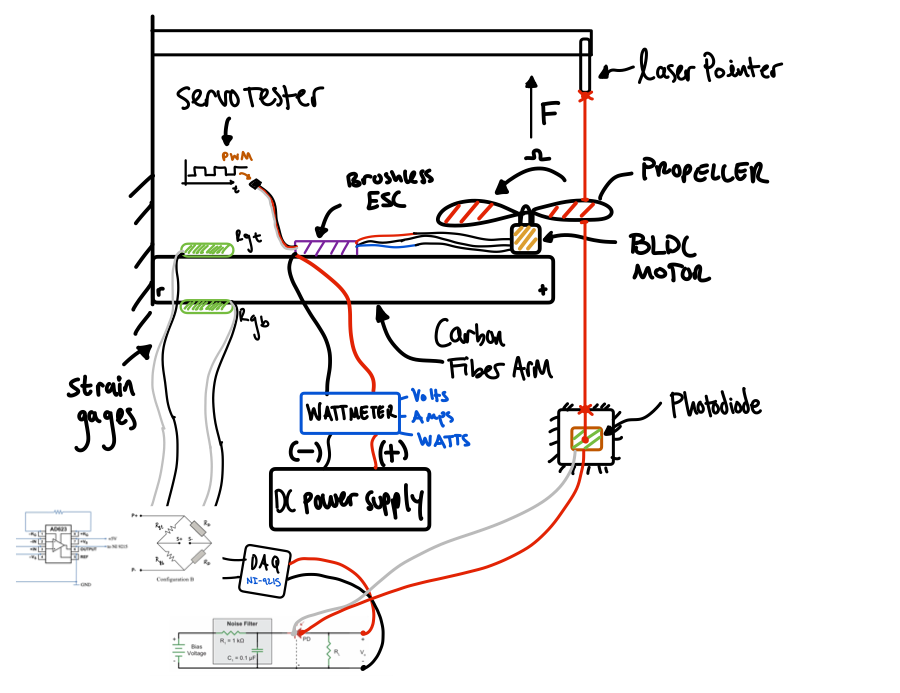
\includegraphics[width = 0.5\textwidth]{finalprojectimages/finalprojectsetup.png}
    \caption{Experiment Setup}
    \label{fig:finalsetup}
  \end{figure}


  \vspace{2.5mm}

  \item Two strain gages, one placed on the top of the carbon-fiber beam and one placed on the bottom. The strain gages will be connected to a DAQ to measure the strain on the beam.
  \item NI-9215 DAQ \hypertarget{7}{[7]} to measure the strain gage and photodiode electrical output.
  \item Instrumentation Amplifier (AD623) \hypertarget{8}{[8]}, to amplify the output of the strain gages and reduce the impact of bias error.
  \item 650nm Laser Pointer (Red). The laser pointer is placed above the propeller offset by 2-3 centimeters from the center and shines through it to hit the photodiode.
  \item Si Photodiode \hypertarget{6}{[6]}, which converts optical power to electrical current. This in concert with the laser pointer will measure the RPM of the propeller, as the propeller will break the beam twice per rotation.
  \item BLDC Motor \hyperlink{1}{[1]} with 20A Brushless Electronic Speed Controller (ESC) \hyperlink{2}{[2]} 
  \item DC Power Supply supplying operational voltage (Replicating 3-Cell Lithium Polymer Battery, 11.1 V), and Watt-meter (\(\epsilon_{b} = 0.05\; \text{W}\)) \hypertarget{9}{[9]}
  \item Servo Tester \hypertarget{5}{[5]} used to send PWM signal to ESC to spin the DC motor at a certain angular rate.
  \item 2 Two-Blade Propellers of 6" diameter and different twist (6x6 \hypertarget{3}{[3]} 6x5.5 \hypertarget{4}{[4]})
  \item Breadboard and wires to connect the circuit. A 10k$\Omega$ resistor, 1k$\Omega$ resistor, and two 350$\Omega$ resistors will be used in the circuit. The two 350 $\Omega$ resistors will be used as dummy resistors for the wheatstone half-bridge configuration (Configuration B used as shown in Lab 5), and the 10k$\Omega$ and 1k$\Omega$ resistors will be used for the photodiode circuit. The full circuit is shown below:
  \vspace{1mm}

  \begin{figure}[H]
    \centering
    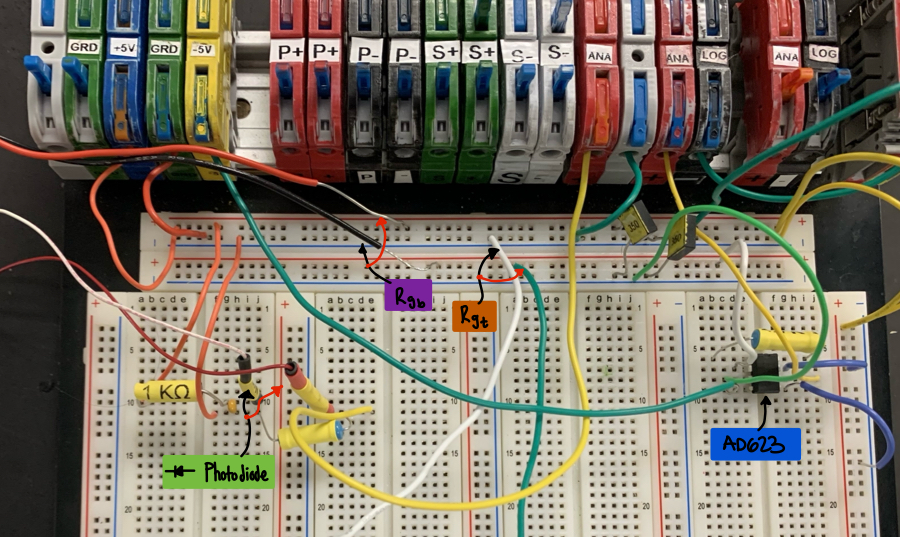
\includegraphics[width = 0.5\textwidth]{finalprojectimages/finalsetupcircuit.jpg}
    \caption{Circuit for Photodiode and Strain Gages}
    \label{fig:finalsetupcircuit}
  \end{figure}

\end{enumerate}

NOTE: To prepare the carbon fiber beam for the strain gages, we sanded down the beam with 80, 120, and 220 grit sandpaper. We then cleaned the beam with isopropyl alcohol and applied the strain gages to the beam with superglue as performed in lab 4. The strain gages were connected to a DAQ and dummy resistors to calibrate the strain gages.
\vspace{1mm}

After some initial testing, the strain gage output was not considered distinguishable from the digitization error. To reduce the impact of this digitization error, we used an amplifier (AD623) to amplify the output of the strain gages.  

\section{Procedure}

\subsection{Strain Gage Calibration}

For calibration, variable brass-slotted weights were placed on the tip end of the cantilevered beam. The strain gage output was recorded at the following weights:
\begin{equation}
    W = [0, 50, 90, 130, 170, 210, 250, 210, 170, 130, 90, 50, 0]
\end{equation}
The half-bridge configuration allows for the linearity to be constant while increasing and decreasing the weights.

\subsection{Trial Procedure}
Before beginning the trials, ensure the LabVIEW model is set up as shown below:
%put labview setup image here

\begin{figure}[H]
  \centering
  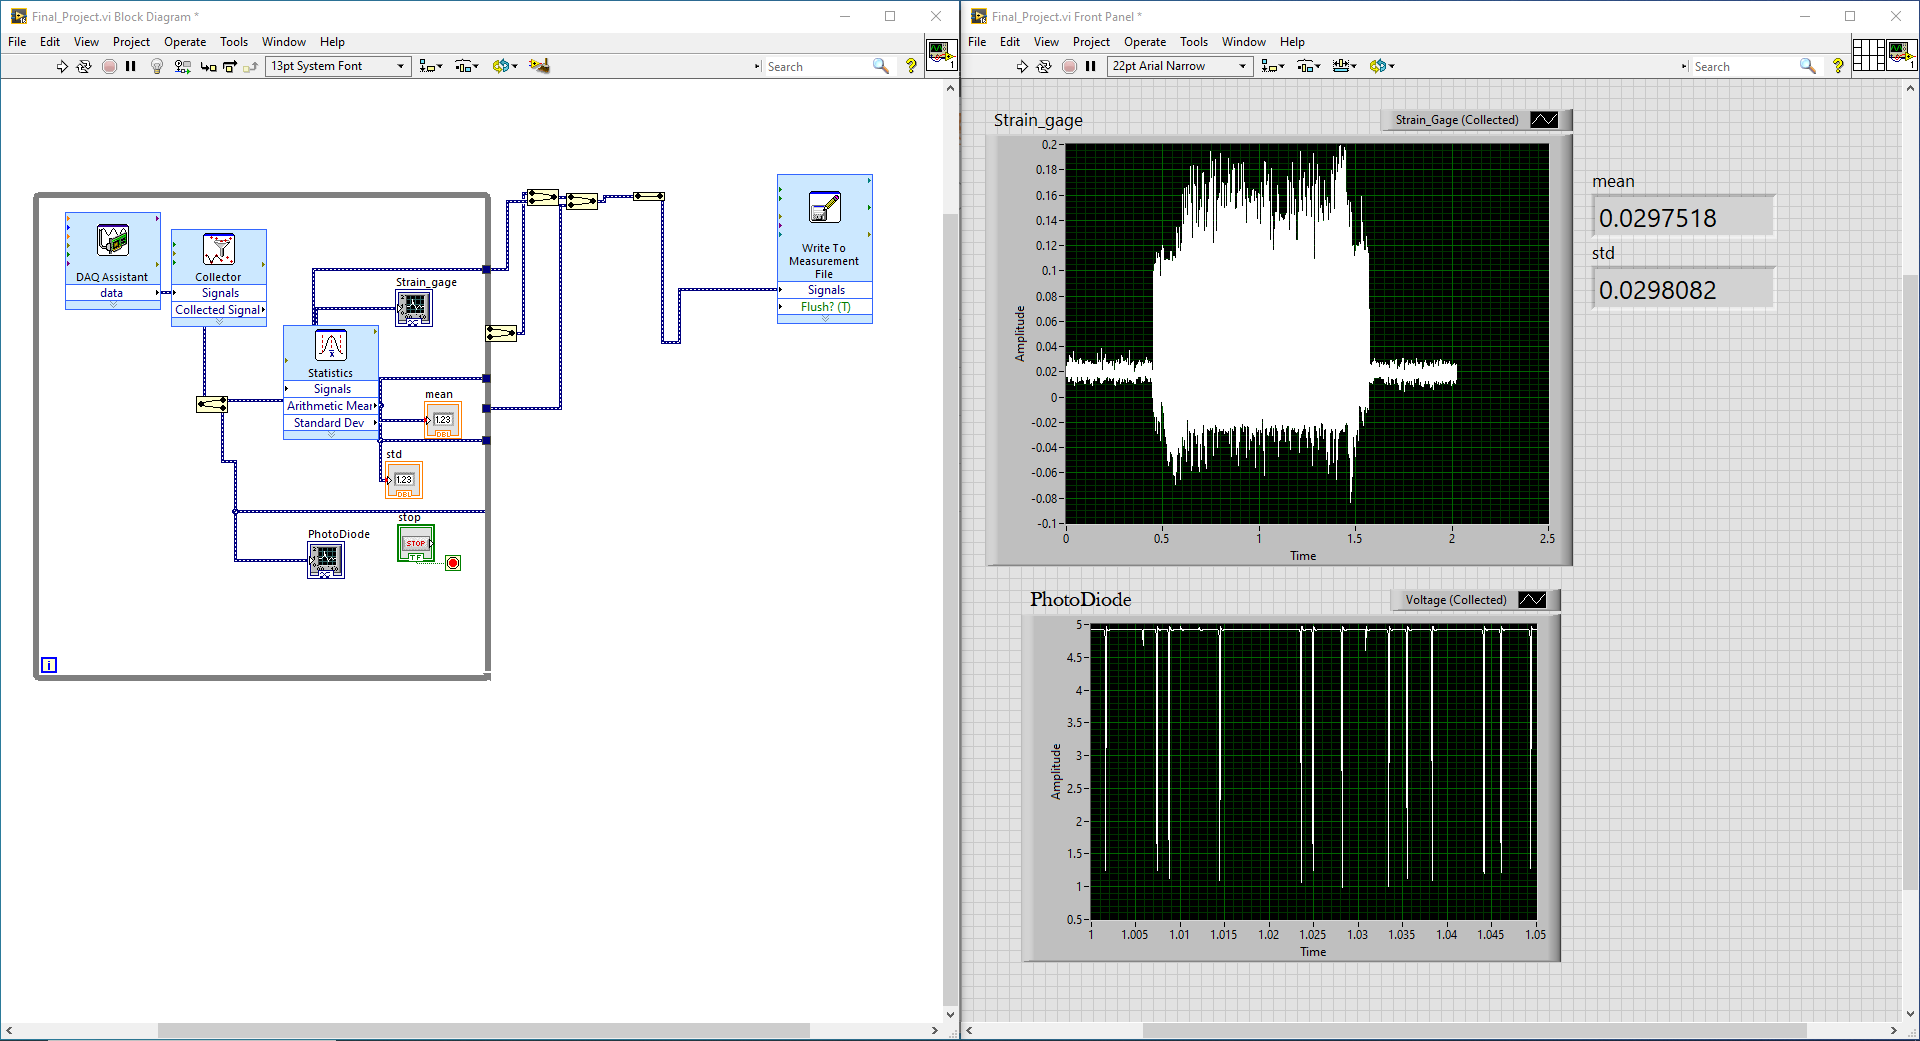
\includegraphics[width = 0.5\textwidth]{finalprojectimages/labviewfinalprojectmodel.PNG}
  \caption{LabVIEW Model for Photodiode and Strain Gages}
  \label{fig:labviewsetupfinal}
\end{figure}

%finish trial procedure
\begin{enumerate}
  \item 
\end{enumerate}

\section{Data Processing}
%add in variables and equations used to calculate theoretical and measured values

\subsection{Variables and Equations}  

Angular Speed, Rotations Per Minute (RPM):
\begin{equation}
    \Omega_{Theoretical} = K_{v}\cdot V_{DC}
\end{equation}
\begin{equation}
    \Omega_{Measured} = \frac{60}{\frac{T}{2}}
\end{equation}

Variables:
\begin{itemize}
    \item \(K_{v}\; \text{RPM/V}\):  RPM a motor will spin at full throttle
    \item \(V_{DC}\): DC Voltage supplied to the motor
    \item \(T\): Period of the Photodiode (seconds)
\end{itemize}

\vspace{5mm}
Thrust-To-Power Ratio
\begin{equation}
    \eta = \frac{m}{W}
\end{equation}

Variables:
\begin{itemize}
    \item \(m\): Mass (grams)
    \item \(W\): Wattage
\end{itemize}
\vspace{5mm}

\section{Results and Analysis}
% SOMEONE PUT STRAIN GAGE GRAPH HERE %

The slope of figure XXX is the ratio at which the strain gage linear increases Voltage as the Force applied increases.  Using the calibration as reference, the ratio can be defined as 
\begin{equation}
   Force_{NEWTONS} = \frac{1}{59638.7} V
   \end{equation}

\begin{figure}[H]
  \centering
  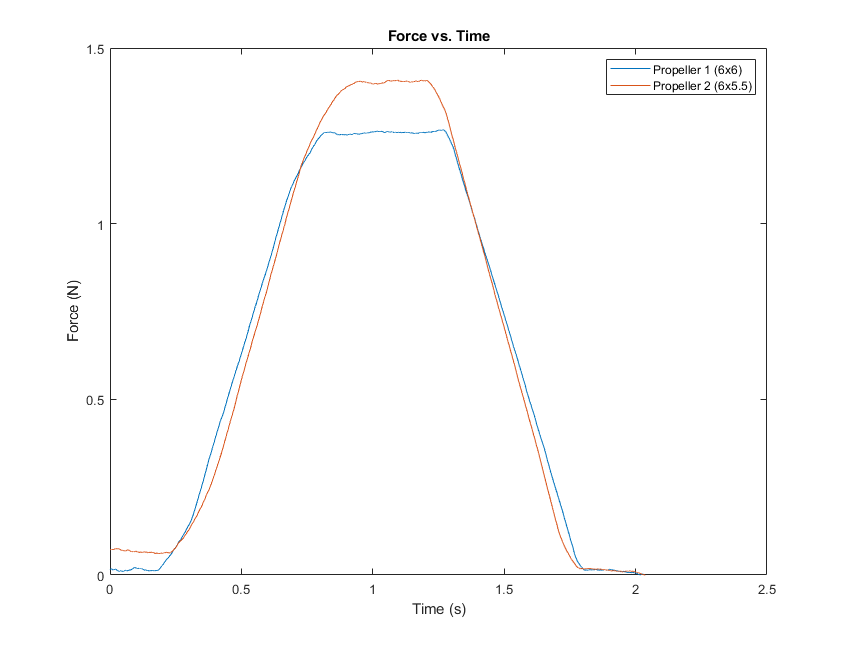
\includegraphics[width = 0.5\textwidth]{finalprojectimages/Trial1_ForcevTime.png}
  \caption{Force vs Time for Trial 1}
  \label{fig:forcevtime}
\end{figure}
% CAN SOMEONE PUT TRIAL 1 AND 2 NEXT TO EACHOTHER INSTEAD OF ON TOP? IDK IF THEY ARE TBH I CANT COMPILE RN
\begin{figure}[H]
  \centering
  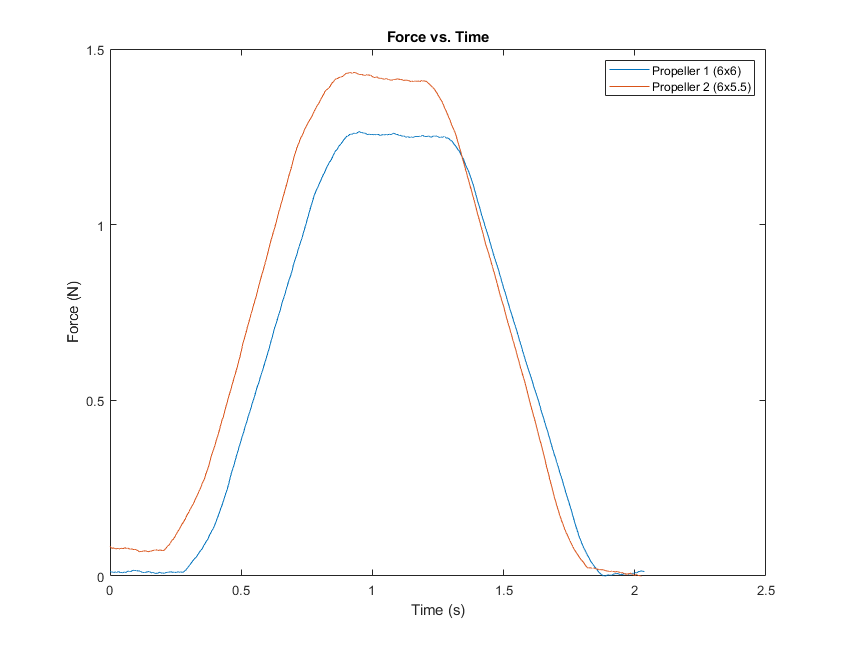
\includegraphics[width = 0.5\textwidth]{finalprojectimages/Trial2_ForcevTime.png}
  \caption{Force vs Time for Trial 2}
  \label{fig:forcevtime2}
\end{figure}

After applying the Calibration Constant to the data with the propellers, a Gaussian filter was used to smooth out the data.  The resultant data was the same in both trials, with the (6x5.5) Propeller providing slightly more thrust than the (6x6) 

\begin{figure}[H]
  \centering
  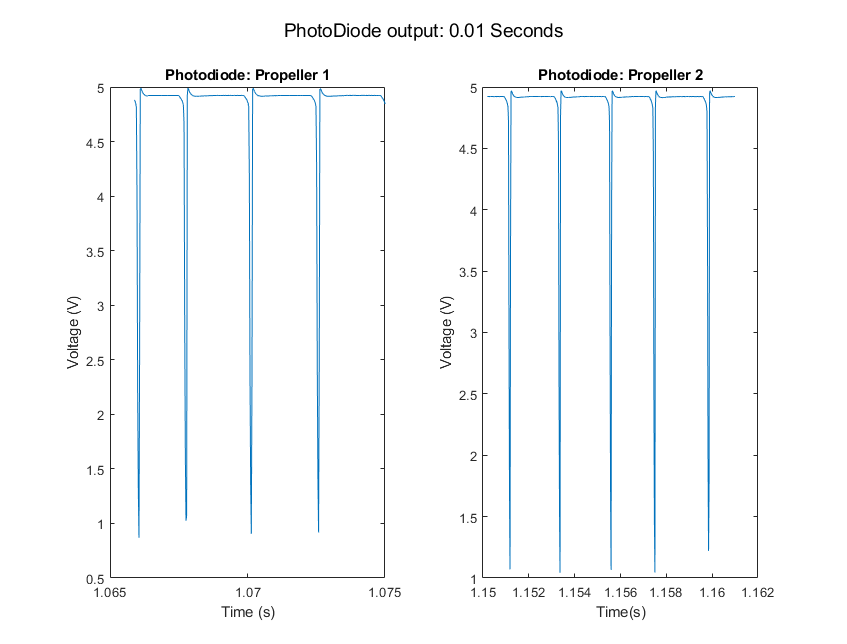
\includegraphics[width = 0.5\textwidth]{finalprojectimages/Trial1_PhotoDiode.png}
  \caption{Photodiode Output for Trial 1}
  \label{fig:photodiode}
\end{figure}

To measure the angular rate of each propeller, the photodiode response was recorded.  The time difference between two consecutive photodiode peaks was considered its period, and since the photodiode responded twice per rotation, the period was divided by 2.  As shown in eq. XX, the periods were calculated and are shown in Table. XXX

\begin{table}[H]
  \centering
  \begin{tabular}{lcc}
  \hline
  \textbf{Parameter} & \textbf{Propeller 1 (6 x 6)} & \textbf{Propeller 2 (6 x 5.5)} \\
  \hline
  Name & 6 x 6 & 6 x 5.5 \\
  RPM (measured) & 26453.2969 & 27705.3444 \\
  RPM (Theoretical) & 26197 & 26990 \\
  RPM (\% error) & 0.97834 & 2.6504 \\
  Force (g) & 129.1952 & 143.6091 \\
  Wattage (W) & 45.55 & 46.7 \\
  Thrust-to-Power (g/W) & 2.8363 & 3.0751 \\
  Uncertainty (\%) & 1.77541 & 1.6756 \\
  \hline
  \end{tabular}
  \caption{Comparison of Propeller Performance - Trial 1}
  \label{table:propeller_comparison1}
  \end{table}

The data from Trial 1 is contained in Table. XX.  The measured RPM for the (6x6) propeller was less than 1\% off of the theoretical, whereas the (6x5.5) propeller was slightly more inaccurate at 2.65\%.  The (6x5.5) Propeller required higher wattage, but produced higher thrust force in return.  The thrust-to-power ratio (g/W) was not significantly affected by the higher wattage, as the (6x5.5) propeller remained slightly more efficient than the (6x6).  
  
\begin{table}[h!]
  \centering
  \begin{tabular}{lcc}
  \hline
  \textbf{Parameter} & \textbf{Propeller 1 (6 x 6)} & \textbf{Propeller 2 (6 x 5.5)} \\
  \hline
  Name & 6 x 6 & 6 x 5.5 \\
  RPM (measured) & 25883.3191 & 26272.3077 \\
  RPM (Theoretical) & 26197 & 26990 \\
  RPM (\% error) & 1.1974 & 2.6591 \\
  Force (g) & 128.9811 & 146.1474 \\
  Wattage (W) & 44.25 & 47.3 \\
  Thrust-to-Power (g/W) & 2.9148 & 3.3028 \\
  Uncertainty (\%) & 1.7554 & 1.674 \\
  \hline
  \end{tabular}
  \caption{Comparison of Propeller Performance - Trial 2}
  \label{table:propeller_performance2}
  \end{table}

Table XX. contains Trial 2.  Nearly every observation made in Trial 1 is also made here.  The force generated by each propeller was nearly identical across both trials, and the uncertainty remained under 2\% for each individual Propeller.  
  
  For Uncertainty in the Thrust to Power ratio, the Wattage, Strain Gage, and DAQ were all sources of error. It was calculated using \begin{equation}
    \epsilon = \sqrt{ \frac{\delta x_1}{x_1}^2 + \cdots + \frac{\delta x_n}{x_n}^2} = \sqrt{ \frac{\delta W}{W}^2 + \frac{\delta \epsilon_{SG}}{\epsilon_{SG}}^2 + (\epsilon_{DAQ})^2}
   \end{equation}
   where \begin{equation}
    \delta W = 0.05 W, \quad \delta \epsilon_{SG} = 0.0002, \quad \text{and} \quad \epsilon_{DAQ} = \frac{5V}{2^{16}-1} 
  \end{equation} 
  % Uncertainty Calculation:  Uncertainty = sqrt( (0.05/Watts)^2 (StrainGage_STD/StrainGageValue)^2 ()^2 (DAQ)^2)

\section{Conclusion}
%Wrap up conclusion


\newpage
\thispagestyle{empty}  % Clear header/footer
\begin{center}
	\vspace*{\fill}
	{\Huge Appendix}
	\vspace*{\fill}
\end{center}

% Start appendices
\newpage
\begin{appendices}
\pagestyle{fancy}
\renewcommand{\thefigure}{A\arabic{figure}}
\setcounter{figure}{0}

\pagebreak

\hypertarget{datasheets}{}
\section{Datasheets}
\begin{enumerate}[label = {[\arabic*]}]
\small
\item \hypertarget{1}{\href{https://hobbyking.com/en_us/multistar-elite-2204-2300kv-multi-rotor-motor-cw-prop-adapter.html}{Multistar Elite 2204-2300KV Multi-Rotor Motor}}
\item \hypertarget{2}{\href{https://hobbyking.com/en_us/afro-20a-race-spec-mini-esc-with-bec.html}{ Afro 20A Race Spec Mini ESC with BEC}}
\item \hypertarget{3}{\href{https://www.apcprop.com/product/6x6e/}{APC 6x6E Propeller}}
\item \hypertarget{4}{\href{https://www.apcprop.com/product/6x5-5e/}{APC 6x5.5E Propeller}}
\item \hypertarget{5}{\href{https://hitecrcd.com/products/servos/discontinued-servos-servo-accessories/discontinued-programmers/hfp-25-digital-servo-programmer-tester-2/product}{HFP-25 Digital Servo Programmer \& Tester}}
\item \hypertarget{6}{\href{https://www.thorlabs.com/drawings/e7e91d1f442ec5dc-834C7101-FD1F-1B62-609D921F0FC0E314/FDS1010-SpecSheet.pdf}{Silicon Photodiode, FDS1010}}
\item \hypertarget{7}{\href{https://www.amc-systeme.de/files/pdf/ni-9215-amc.pdf}{NI-9215 Datasheet}}
\item \hypertarget{8}{\href{https://www.analog.com/media/en/technical-documentation/data-sheets/ad623.pdf}{AD623 Instrumentation Amplifier Datasheet}}
\item \hypertarget{9}{\href{https://www.amazon.com/Analyzer-Digital-Balance-Battery-Voltage/dp/B0753DPC2D/ref=asc_df_B0753DPC2D/?tag=hyprod-20&linkCode=df0&hvadid=309806250188&hvpos=&hvnetw=g&hvrand=1339579772044864897&hvpone=&hvptwo=&hvqmt=&hvdev=c&hvdvcmdl=&hvlocint=&hvlocphy=9028280&hvtargid=pla-567839154382&psc=1&mcid=0273f08627a23b188506d62979b40559&gclid=CjwKCAjw57exBhAsEiwAaIxaZg9oUrMDzZ3wh-Y_MJXKuUsgDDHnvtvx1OtjC213FpZroDuJ3cO4sBoCM-YQAvD_BwE}{RC Watt Meter DC 60V/100A }}
\end{enumerate}

\end{appendices}

\end{document}
